\chapter{Design and Application} 

\label{chapter4}

The design of the \acrfull{ssdr} along with the \acrfull{prc} and its subsequent application for implementing the research aim is presented in detail in this chapter. As usual in the research design \textit{case study}, the results partly build on each other and evaluations had to be made in the intermediate steps to allow further continuation. This results-centred chapter will therefore also have small parts of further explanations and discussions of interim results, to allow the flow of thought to follow the decisions made. Nonetheless, these parts were kept to the bare minimum, leaving major discussions to the next chapter.\newline 
In the opening section, the newly developed \ref{sec:ssdr} for community-based participatory mapping and monitoring of water sources for water-scarce and resource-limited settings to facilitate relevant AAs in the context of FbF addresses the first research question. The developed \acrlong{ssdr} is a highly adapted and extended version of the \acrshort{ssf} taking into account the setting of the case study area, the research context and several other guidelines. The \acrlong{ssdr} is further accompanied by the also newly developed \acrshort{prc}, which is presented in section \ref*{sec:prc} of this Chapter. The interplay between the \acrshort{ssdr} and the \acrshort{prc} can be seen in figure \ref{fig:res_ssdr_prc}. Section \ref{sec:f_a} addresses the second research question by presenting the created implementation roadmap for a practical project in Somaliland, which resulted from the application of the new \acrshort{ssdr} together with the \acrshort{prc} on the Somaliland context.\newline
The data used are listed in Appendix \ref{AppendixA} and the full interview and questionnaire transcripts can be found in Appendix \ref{AppendixB}. The chapter concludes with a short summary containing the main findings.


\section{Six Stage Design Roadmap}\label{sec:ssdr}
The six stages of the \acrshort{ssdr} are presented in the coming sections. The design of the roadmap is primarily oriented on the \acrshort{ssf} but additionally incorporates several other \acrshort{cs} project guidelines and experiences, information from the conducted interviews, and the wider literature. While the stages conceptually separate the design process, it is important to keep in mind, that the stages are interconnected and in particular stages 3 to 6 can and should be worked on to some extent in parallel or iteratively. Stages 1 and 2 are primarily important in the beginning and when major changes of goals or conditions take place during the design, implementation or operation phase. Thus, once the first two stages are successfully conducted, the actual design procedure will be an iterative process, that mainly incorporates these last 3 to 6 stages. This, and its interplay with the \acrshort{prc} can be seen in figure \ref{fig:res_ssdr_prc}\newline

\missingfigure{New and awesome, if not to say marvelous depiction of this, the universe and the meaning of life. Just day to day stuff ya know.}
\begin{figure}[!htp]
    \centering
    \includegraphics[width=0.9\textwidth]{figures/}
    \decoRule
    \caption[Drought Sequences]{}
    \label{fig:res_ssdr_prc}
\end{figure}


Stage 1 outlines the exploration phase to establish a first understanding of the problem, context and potential solutions. The second stage elaborates on how to conduct a feasibility study to evaluate the \acrshort{cs} approach regarding the identified problem in the given context. When the feasibility of the \acrshort{cs} approach is confirmed, the overall structure of the project is laid out in Stage 3 \textit{Designing the Project}. This stage describes the usage of the gathered information of stage 1 and 2 to further specify the research goal, respective products to reach these goals and the activities that constitute to the products. More guidance is given to which additional data needs to be collected, assessed and integrated to lay a good foundation for the coming stages. Stage 4 is concerned about topics surrounding community building efforts and Stage 5 outlines concerns in regard to data management. The last Stage, \textit{Stage 6 Evaluation and Iterative Improvements} underlines the importance and elaborates on the practical implementation of ongoing assessment and improvement measures.

\subsection{Stage 1: Context \& Problem Identification}\label{subsec:stage1_design}

This first Stage is the exploration phase of the overall project \autocite{citizenscience.govBasicStepsYour}. This is where the environment of this project is established, in which itself is embedded. It is aimed at identifying prevailing conditions in all areas that may be covered or touched by the project. Even if this stage does not go into too much detail, the identification efforts must be thorough and as complete as possible. Oversights in this stage can have serious consequences in later stages. To enable this identification, project boundaries must first be defined by the overall objective and the problems to be solved, which also take into account challenges, positive and negative constraints as well as resource requirements. In addition, potential key stakeholders should be involved from the beginning and comparable projects and data sets need to be carefully identified and analysed to avoid duplication \autocite{citizenscience.govBasicStepsYour,fraislCitizenScienceEnvironmental2022,minkmanCitizenScienceWater2015}. Based on this information, possible solutions can be derived and hypotheses or research questions formulated \autocite{silvertownNewDawnCitizen2009}. Additionally, evaluation practices and sustainability considerations should be integrated into the project as early as possible although they are only defined in detail at a later stage \autocite{fraislCitizenScienceEnvironmental2022}.

\subsection{Stage 2: Citizen Science Feasibility Assessment}\label{subsec:stage2_design}

The \acrlong{cs} approach is not feasible for all kinds of projects. Certain criteria should be met and the feasibility of design, implementation and operation must be ensured and tailored to the decision-making processes that the project aims to influence. Fundamentally, a \acrshort{cs} project must contribute to achieving the defined objectives and solving the problems, while also providing benefits to the participants, e.g. in terms of knowledge, community or recreational value \autocite{escaeuropeancitizenscienceassociationTenPrinciplesCitizen2015}. The feasibility assessment needs to consider various factors and constraints in more detail than in Stage 1 to identify information and management gaps accordingly. The clear definition of the relevant \acrshort{cs} sub-concepts and levels of participation is crucial for the feasibility assessment. It is also important to clearly outline the boundaries and concepts by which and within which the project is to be confined and embedded. The goal should be clarified along with potential sub-goals and related products which need to match the derived gaps and the capacity of the implementing organisation \autocite{ifrcCommunityBasedSurveillanceGuiding2017,minkmanCitizenScienceWater2015}. The organisational capacity depends on financial, human and technical resources, knowledge and experiences, embedding in decision-making networks and structures, and the organisational commitment and dedication of those involved \autocite{fraislCitizenScienceEnvironmental2022,ifrcCommunityBasedSurveillanceGuiding2017}. The importance of securing (long-term) funding is also highlighted by many guidelines \autocite{cervoniImplementingIntegratedWater2008,minkmanCitizenScienceWater2015,sharpeCommunityBasedEcological2006, whitelawEstablishingCanadianCommunity2003}. Existing data sets and potential tools need to be analysed and assessed for suitability. In addition to the positive constraints, the \textcite{ifrcCommunityBasedSurveillanceGuiding2017} has defined negative \textit{red flag} constraints which, when they occur, should stop further design developments until they can be resolved appropriately. Going back to the exploratory Stage 1 to explore and evaluate the issue may be necessary if a \textit{red flag} should be reached. The adapted \textit{red flags} are:

\begin{itemize}
    \item A need does not exist.
    \item The community does not want the project.
    \item Barriers and fears of: information usage, data sharing, applied technology and different cultural beliefs.
    \item Insufficient capacities regarding financial and human resources, knowledge, experience and phone coverage.
    \item No support of key stakeholders.
    \item No or insufficient response possibilities.
\end{itemize}
\hfill {\footnotesize Based on \textcite{ifrcCommunityBasedSurveillanceGuiding2017}}

\subsection{Stage 3: Structure \& Design}\label{subsec:stage3_design}
This stage builds on the identified context and conditions of stage 1 and the feasibility study of stage 2 and creates the broader framework for more specific work in Stages 4, 5, and 6. The goals and research questions are considered again and finally specified and formulated in alignment with the projects, participants and stakeholders interests and aims \autocite{conradReviewCitizenScience2011,minkmanCitizenScienceWater2015}. Previous assumptions should be backed up as much as possible and made explicit \autocite{silvertownNewDawnCitizen2009} and biases need to be addressed \autocite{escaeuropeancitizenscienceassociationTenPrinciplesCitizen2015,fraislCitizenScienceEnvironmental2022}. "Legal and ethical issues surrounding copyright, intellectual property, data sharing agreements, confidentiality, attribution, and the environmental impact of any activities" (principle 10, \textcite{escaeuropeancitizenscienceassociationTenPrinciplesCitizen2015}) need to be considered. The design need to be thoroughly embedded in the context and anchored by policies, preferably in an \acrlong{iwrm} initiative \autocite{cervoniImplementingIntegratedWater2008,sharpeCommunityBasedEcological2006} and ongoing \acrshort{fbf} implementations and efforts. The 'light' \acrshort{iwrm} \textit{community-based water resource management} framework by \autocite{dayCommunitybasedWaterResources2009} is recommended as a starting point as it is geared towards practical feasibility (see section \ref{subsubsec:groundwork}). The integration into the \acrshort{fbf} is done by targeting data management (stage 5) on indicators which support intended triggers and respective anticipatory actions \autocite{ifrcCommunityBasedSurveillanceGuiding2017}. Adequate and scientifically justified thresholds and monitoring methods may need to be developed and triangulation data sets identified, assessed and integrated. \newline
A structured and interconnected foundation needs to be created for the integration of communities and stakeholders (Stage 4), data management (stage 5) and evaluation and iterative improvement procedures (stage 6). Community building encompasses recruitment, training, task specifications and participant benefits, motivations, feedback mechanisms and stakeholder acknowledgements. It is also concerned with the broader frame of partaking and collaborating non-governmental organisations and government bodies at all levels \autocite{conradReviewCitizenScience2011}. Data management practices should be oriented on already proven concepts of comparable projects, identify and define data collection, transmission, storage and analysis aims, formats, and types \autocite{fraislCitizenScienceEnvironmental2022,gualazziniEWEAEarlyWarning2021,ifrcCommunityBasedSurveillanceGuiding2017}. Consideration also needs to be given to the ways in which the new data from this project can be publicly displayed, accessed and used to improve completeness, timeliness and overall quality of information and decision-making processes \autocite{conradMeaningfulCommunityBasedEcological2006}. Evaluation and iterative improvement procedures are concerned with pre-defining success metrics which should be considered during the entire project design and operation.\newline
In this third stage, the project requirements catalogue presented in the coming section \ref*{sec:prc} is recommended for integration to reduce mental load in the further design process.

\subsection{Stage 4: Community \& Stakeholder}\label{subsec:stage4_design}

This section pertains to the identification and establishment of all relevant factors associated with the participants, community, network, and organizational and governmental stakeholders and decision-makers. Understanding participants characteristics and motivations as primary data collectors and contributors to the project is of great importance for the sustainable success of the project. Their characteristics can include, among others, the educational level, skills and demographics \autocite{cervoniImplementingIntegratedWater2008,fraislCitizenScienceEnvironmental2022}. The motivational aspects comprise elements of interest, engagement, acknowledgements and overall gained benefits. The first set of characteristics can be addressed by training, supervision and provision of feedback, especially for new participants \autocite{escaeuropeancitizenscienceassociationTenPrinciplesCitizen2015,fraislCitizenScienceEnvironmental2022,minkmanCitizenScienceWater2015,sharpeCommunityBasedEcological2006}. Providing feedback to the actual contributions but also in terms of how the contributions influence planning and management decision-making processes and outcomes can positively influence the motivational aspects \autocite{conradMeaningfulCommunityBasedEcological2006,conradReviewCitizenScience2011,whitelawEstablishingCanadianCommunity2003}. Creating wider public engagement and interest can further enhance motivational factors such as recognition and community building \autocite{conradMeaningfulCommunityBasedEcological2006}. Community events and networking bring further social benefits, trust and belonging and open up opportunities to engage directly with decision-makers and make them aware of what this project is and why it exists \autocite{conradMeaningfulCommunityBasedEcological2006,fraislCitizenScienceEnvironmental2022,sharpeCommunityBasedEcological2006}. Decision-makers, such as respective water and risk related government ministries and agencies, should be integrated in the process and design right from the beginning as especially local and regional leaders can help to implement and operate the project on site \autocite{gualazziniEWEAEarlyWarning2021,ifrcCommunityBasedSurveillanceGuiding2017}. They can furthermore help to sensitize the community, manage expectations and inform about and support in dealing with oppositely motivated stakeholders (I1). \autocite{conradMeaningfulCommunityBasedEcological2006} encourages the perspective of integrating the project into the management as an opportunity and not as a threat. Inclusion of legal and ethical guidelines should also happen in this stage, but has its focus in the upcoming stage 5 \autocite{fraislCitizenScienceEnvironmental2022, ifrcCommunityBasedSurveillanceGuiding2017,minkmanCitizenScienceWater2015}.

\subsection{Stage 5: Data Management}\label{subsec:stage5_design}

Legal and ethical laws, guidelines, and standards especially in terms of privacy and data security need to be respected. This also includes taking into account informal, community and cultural practices during all phases of data management \autocite{ifrcCommunityBasedSurveillanceGuiding2017}. These phases encompass the planning and design, the collection on site, the transmission, storage, \acrfull{qa} and \acrfull{qc} as well as subsequent analysis, presentation and dissemination of the outcomes \autocite{fraislCitizenScienceEnvironmental2022}.\newline
All of these phases need to match the capacities of the organisation and of the contributing participants \autocite{ifrcCommunityBasedSurveillanceGuiding2017,minkmanCitizenScienceWater2015}. Furthermore, all practices should focus on the end use and application of the data in supporting decision-making and follow the principle of data minimisation \autocite{edpsGlossaryEuropeanData2023,ifrcCommunityBasedSurveillanceGuiding2017,minkmanCitizenScienceWater2015}. In this stage, the planning of the data management procedures enters its detailed phase, is based on the established structure in Stage 3 and results in precise methods, techniques, protocols and scripts. The methods should be simple, well-designed, peer-reviewed and standardised, while being fit for purpose \autocite{fraislCitizenScienceEnvironmental2022,ifrcCommunityBasedSurveillanceGuiding2017,silvertownNewDawnCitizen2009,whitelawEstablishingCanadianCommunity2003}. \acrshort{qa} and \acrshort{qc} procedures should ideally be integrated in every phase and follow the same high standards as the methods \autocite{fraislCitizenScienceEnvironmental2022,mackechnieRoleBigSociety2011,sharpeCommunityBasedEcological2006,silvertownNewDawnCitizen2009}. Financial and human investments and resources need to be specified and parameters about the technical infrastructure such as architecture, storage, analysis, transmission and collection protocols and methods need to be defined \autocite{fraislCitizenScienceEnvironmental2022,sharpeCommunityBasedEcological2006}. For data collection "the least intrusive and most cost-effective method available" (p.27) is recommended \autocite{ifrcCommunityBasedSurveillanceGuiding2017}. The applied tools for data collection and transmission need to meet the available resources and technical abilities of the participant on site \autocite{ifrcCommunityBasedSurveillanceGuiding2017,minkmanCitizenScienceWater2015}. Network coverage should be taken into account when implementing SMS or other remote devices but the \textcite{ifrcCommunityBasedSurveillanceGuiding2017} notes, that "it is now increasingly rare to have absolutely no network access, but a bicycle messenger or another local communication system will also work" (p.26). An automated, technical remote solution should be the preferred solution, but simple SMS and phone calls directly to the relevant manager or via traditional communication networks can also work, especially in cases where transmission speed is not of utmost importance \autocite{gualazziniEWEAEarlyWarning2021,ifrcCommunityBasedSurveillanceGuiding2017}. The requirements for data storage solutions include secure storage, good maintenance options and high up-times. The position of the servers and the ownership of the data can lead to disagreements with local stakeholders and should be well communicated (I2). Before the analysis of the data, robust \acrshort{qa} and \acrshort{qc} measures should ensure high quality of the collected data \autocite{fraislCitizenScienceEnvironmental2022,sharpeCommunityBasedEcological2006}. The integration of other data sources for information triangulation is recommended. The analysis is the centrepiece of the data management and should follow the objectives of the overall project. The outcomes should be made publicly available unless prevented by security or privacy concerns \autocite{escaeuropeancitizenscienceassociationTenPrinciplesCitizen2015,sharpeCommunityBasedEcological2006}. The type of presentation can show aggregated data, but should take into account the information needs of decision-makers. As with the issue of ownership of data, the procedures for sharing and presentation can also lead to disagreements and need to be managed sensitively (I3; \cite{ifrcCommunityBasedSurveillanceGuiding2017}).

\subsection{Stage 6: Evaluation \& Iterative Improvements}\label{subsec:stage6_design}

Evaluation is an ongoing effort and should be considered at all phases of the project. The structure of the project should allow for evaluation procedures and subsequent implementation of the derived recommendations at all design stages and during operation \autocite{fraislCitizenScienceEnvironmental2022,ifrcCommunityBasedSurveillanceGuiding2017}. Success metrics as well as the response upon those need to be defined and agreed upon before the implementation of the project \autocite{fraislCitizenScienceEnvironmental2022,gualazziniEWEAEarlyWarning2021}. The ninth principle of \textcite{escaeuropeancitizenscienceassociationTenPrinciplesCitizen2015} states, that "citizen science programmes are evaluated for their scientific output, data quality, participant experience and wider societal or policy impact" (principle 9). Underlying structures, practices and efforts can thus be configured and adapted into a more effective and efficient design and process. The integration of these assessments thus helps to progressively improve the use of data by decision-makers as well as the methods used \autocite{fraislCitizenScienceEnvironmental2022}.


\section{Project Requirements Catalogue}\label{sec:prc}

The \acrfull{prc} extends the process-oriented structure of the \acrshort{ssdr} by listing, structuring and grouping important information requirements in line with their inter-dependencies. The catalogue of project requirements presented here is divided into four groups of information that include \citeauthor{minkmanCitizenScienceWater2015}'s \citeyear{minkmanCitizenScienceWater2015} derived goals and sub-goals and follows the layer structure of the \acrshort{slmc}. For each goal, products along with their required activities have been defined in line with the above roadmap.\newline
The first group \textbf{Knowledge Base}, see figure \ref{fig:res_knowledge}, contains everything that should be known for the project. It thereby serves as a knowledge base being filled throughout the above-mentioned stages. Activities are primarily about identification and information collection. The second group \textbf{Groundwork} contains everything on which the actual implementation of the project must be based on, see figure \ref{fig:res_groundwork_ar} and \ref{fig:res_groundwork_pd}. It includes the goals \textit{Awareness Raising, Public Education and Policy Development}. The first two goals relate to products of information and sensitization measures for the target community, contributing volunteers and involved stakeholders. Activities focus on consulting with local elders and key stakeholders, and subsequently informing and raising awareness among the entire community before the project starts. The third goal, \textit{Policy Development} is about \acrshort{iwrm} measures, required products and their development. The activities aim to embed these into existing local management practices and procedures through identification and agreements with all affected and involved stakeholders. In order to facilitate this, new policy developments and adjustments may be required which overlap with the third group of \textbf{Innovations}, see figure \ref{fig:res_innovations}. This stage is important, as "there is no one-size-fits-all approach" \autocite[2]{fraislCitizenScienceEnvironmental2022} and new developments of suitable and scientifically sound methods to meet specific challenges of the project tasks will be necessarily in nearly every application to some extent and are summarised under the goal of \textit{Method Improvements}. The last group \textbf{Management} contains all that needs to be done to successfully develop and implement a \acrshort{cs} water source mapping and monitoring project, see figure \ref{fig:res_management}. The goal \textit{Management Improvements} is further subdivided into products that are initially necessary once, recurrently and products that are required to embed the project in the context. The focus of the activities is on making decisions, developing procedures based on the \textbf{Groundwork} and \textbf{Knowledge Base} groups and implement developed methods from the \textbf{Innovations} group.\newline
The order of the sections does not necessarily reflect the processing order but rather indicates dependencies whereas e.g. not everything need to be known in order to proceed with method development. The same applies to the order of products and activities (from top to bottom). However, to stay in this example, everything that, directly or indirectly, influences or is influenced by this certain method should be known. Therefore, stages 1 and 2 of the \acrshort{ssdr} should be completed before proceeding further with this catalogue in order to have a profound understanding of the local circumstances and their interconnectedness and interdependences.\newline
The following sections briefly reason and describe the overall idea and content of each group. The activities are mostly already outlined in the above-described \acrshort{ssdr}, therefore the focus lies on the products of each goal. 

\subsection{The Knowledge Base: What needs to be known}\label{subsubsec:knowledge}

This Knowledge Base covers information and knowledge of all stages and is sub-divided into multiple products that each cover certain aspects of the project. The products (A), (B), (C) and (D) cover the baseline information of all stages. (A) includes information obtained in Stages 1 and 2 and, if this project is developed under an EAP, also the information from the overarching EAP assessment and feasibility study can be integrated. (B) is the repository for all information related to the \acrlong{cs} community and participant management, (C) covers all topics of data management and \acrshort{qc} and \acrshort{qa} integration and (D) relates to evaluation and improvement procedures. These products consciously resemble Stages 4, 5 and 6, and should be included right at the beginning of Stage 3. The structural basis for each of the subsequent stages is laid in Stage 3, and by bundling the information from the beginning, follow-up in the subsequent stages is simplified and streamlined.\newline

\begin{figure}[!htp]
    \centering
    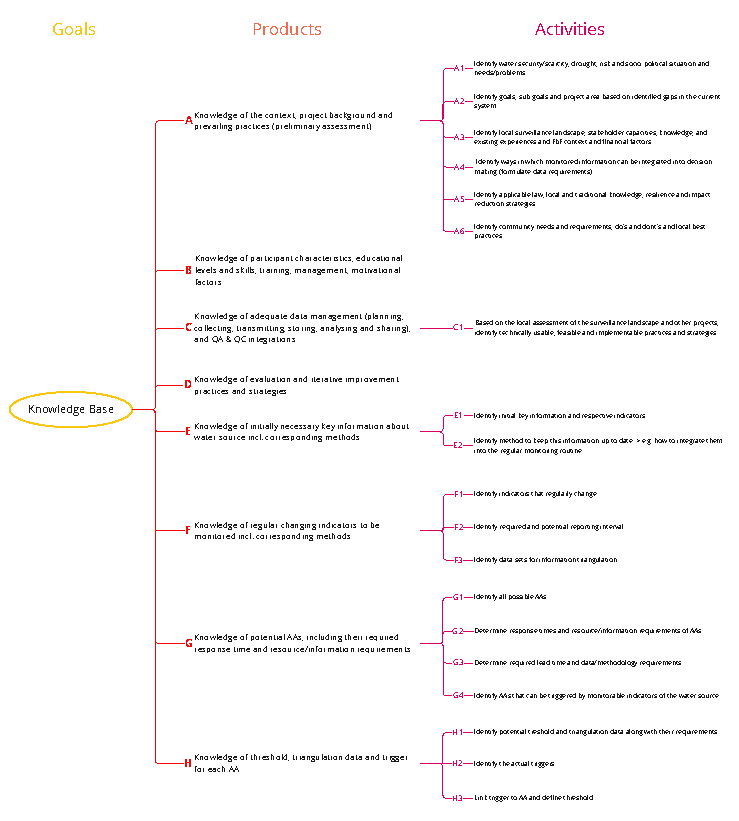
\includegraphics[width=1.0\textwidth]{figures/2023_MA_results_knowledge.pdf}
    \decoRule
    \caption[PRC: The Knowledge Base]{The Knowledge Base. Source: Own representation.}
    \label{fig:res_knowledge}
\end{figure}

Products (E) to (H) are more specific for the mapping and monitoring of water sources in an \acrshort{fbf} context. (E) integrates all information for the first phase of mapping and collection of key information on each water source including corresponding methods, while (F) includes all knowledge and methods on regular indicator monitoring. Together, this information enables actions on products (G) and (H). All potential \acrshortpl{aa} are first collected in product (G) and then narrowed down to those that can be triggered by thresholds related to water sources. The information about these thresholds along with triangulation data for the respective triggers is comprised in product (H).


\subsection{The Groundwork: What needs to be built on}\label{subsubsec:groundwork}
The Groundwork relates to everything, that needs to be in place, before the actual mapping and monitoring of the water sources starts. It is about giving the community all the information and knowledge to decide, manage and act primarily on their own, ideally only limited by the available physical and financial resources. Important is, that knowledge should not opposed on the communities but rather developed in close cooperation with the affected actors, their knowledge and practices. The first product (A) of the goals \textit{Awareness Raising \& Public Education} (see figure \ref{fig:res_groundwork_ar}) is about gathering and then providing all the necessary background information to the community in order to allow them to make profound and informed decisions and contributions. Based on this, product (B) summarizes activities to address misunderstandings, reservations as well as expectations and concern handling. For this, the early involvement of community leaders or elders may be beneficial (I1). Product (C) refers to the sharing of information gathered in other phases with the community to keep their knowledge of prevailing and evolving circumstances up to date and to enable informed decision-making. In order to act on the information, product (D) summarizes the identification and transfer of information about water management and saving opportunities. Product (E) highlights the consideration, that even a single community is not homogeneous and that various groups with different interests exist within. Knowledge and measures to account for this are collected under this product.\newline

\begin{figure}[!htp]
    \centering
    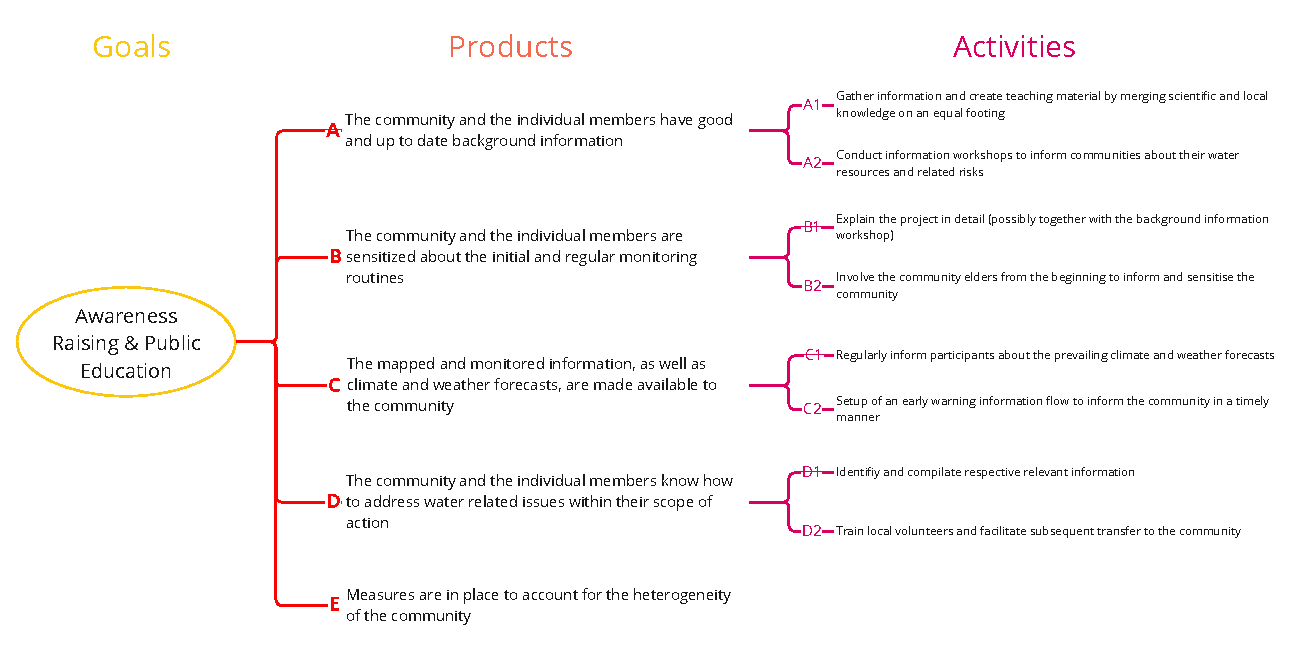
\includegraphics[width=1.0\textwidth]{figures/2023_MA_results_awareness.pdf}
    \decoRule
    \caption[PRC: The Groundwork - Awareness Raising \& Public Education]{The Groundwork: Awareness Raising \& Public Education. Source: Own representation.}
    \label{fig:res_groundwork_ar}
\end{figure}

Products A to E of goal \textit{Policy Implementation}, figure \ref{fig:res_groundwork_pd}, represent \citeauthor{dayCommunitybasedWaterResources2009}'s \citeyear{dayCommunitybasedWaterResources2009} light community-based \acrshort{iwrm} framework. The framework starts with the products (A) \& (B) by identifying and assessing prevailing circumstances and requirements. From this, community water usage targets are derived and agreed upon in (C). Management guidelines, and prioritisation plans are pre-defined and implemented in products (D) and (E). Product (F) goes beyond the framework and addresses measures related to data security and privacy.

\begin{figure}[!htp]
    \centering
    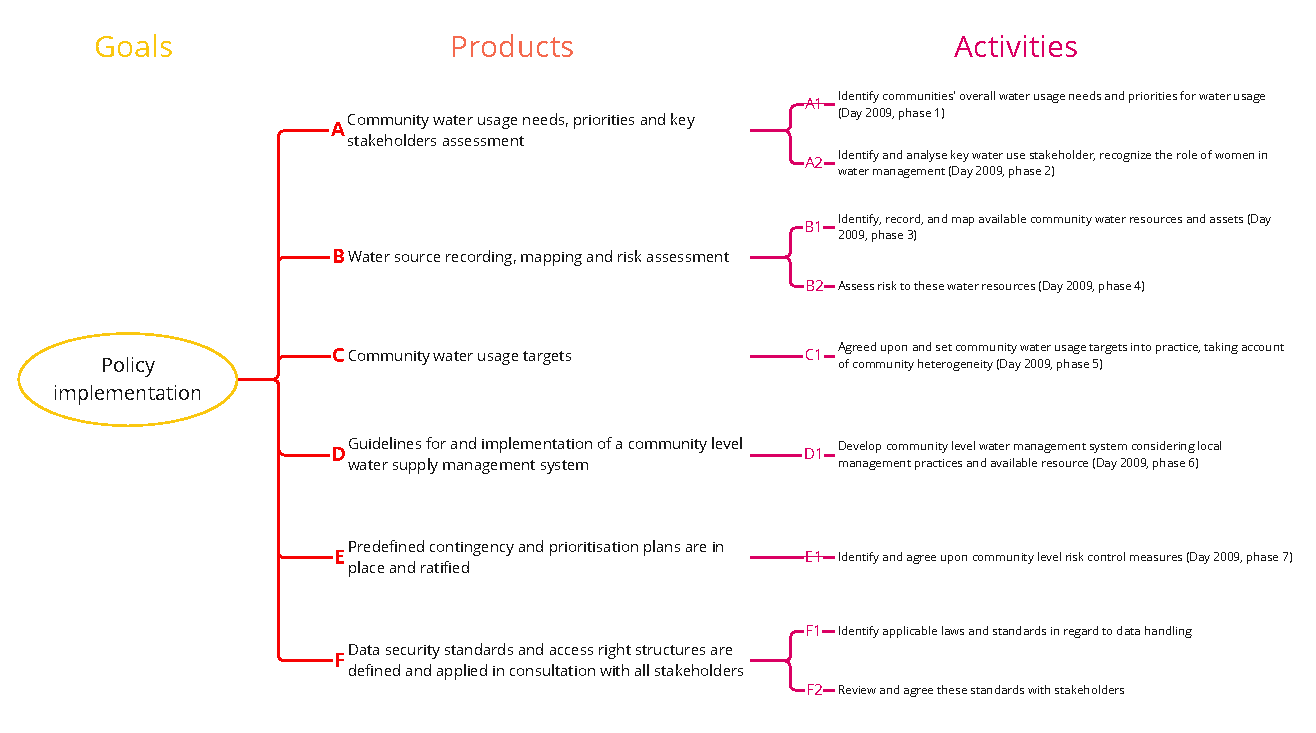
\includegraphics[width=1.0\textwidth]{figures/2023_MA_results_policy.pdf}
    \decoRule
    \caption[PRC: The Groundwork - Policy Development]{The Groundwork: Policy Development. Source: Own representation.}
    \label{fig:res_groundwork_pd}
\end{figure}

\subsection{The Innovations: What needs to be invented}\label{subsubsec:innovations}
New innovations may be required to successfully achieve the project objectives under the given conditions and in the given context. These developments are grouped separately because the development of appropriate, scientifically sound and context-aware methods can require a great deal of financial, material and human resources and should therefore receive specific consideration. In addition, the development of new methods is often a separate process that runs alongside the actual design and implementation efforts. However, there are now also many projects, guidelines and frameworks from which experience and best practices can be transferred. The developments can therefore also be an amalgamation of the old, tailored to new circumstances.\newline

\begin{figure}[!htp]
    \centering
    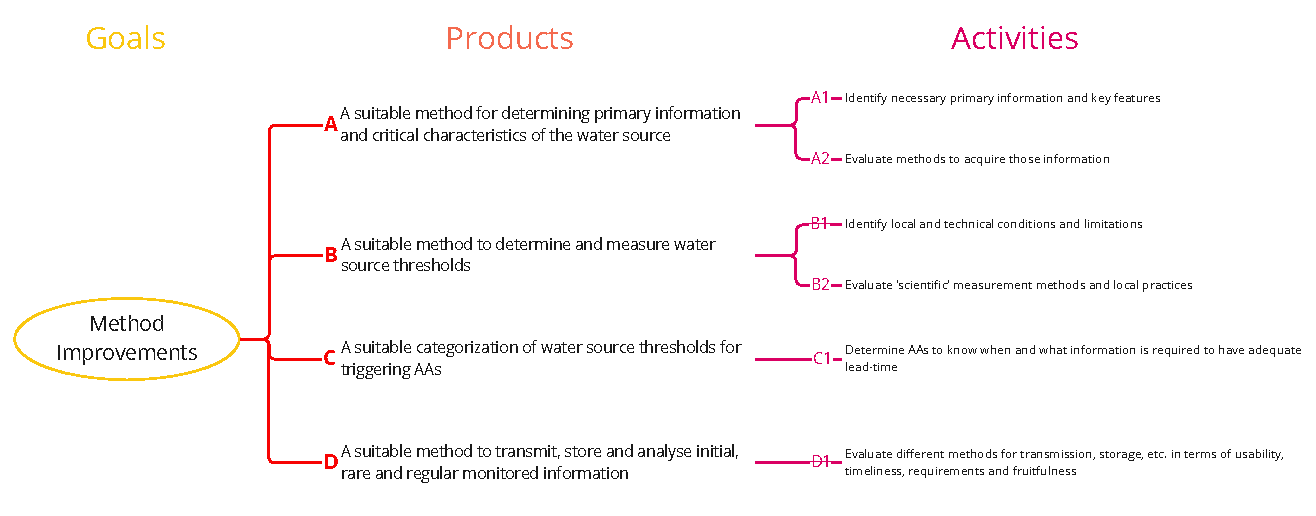
\includegraphics[width=1.0\textwidth]{figures/2023_MA_results_innovation.pdf}
    \decoRule
    \caption[PRC: The Innovations]{The Innovations. Source: Own representation.}
    \label{fig:res_innovations}
\end{figure}

The products represent potential areas of such required innovations or adaptations. These can include areas of the initial and regular data collection, transmission, storage and analysis as well as, the determination of suitable thresholds, and their categorization for respective triggers.

\subsection{The Management: What needs to be done}\label{subsubsec:management}
The group around management tasks is primarily concerned with the initial processes and responsibilities at the start of the project, tasks that need to be done regularly during operation, and specifications for solidly embedding the project in prevailing processes and practices. These tasks are about evaluating and processing identified and collected information to develop and make decisions about what elements, practices or structures to implement. The initial areas of concern (A) range from handling specific context related circumstances, to the development of training materials and evaluation procedures. Activities contributing to regular required products (B) are mostly concerned about providing training and supervision and implementing improvements derived from evaluations and feedback. Product (C) includes both initial and ongoing tasks, but is focused on embedding the project in the local context. It addresses the implementation of the \textit{Groundwork} on community level and its integrations into prevailing local, regional and national structures, practices and stakeholder networks to make it relevant for decision-making.

\begin{figure}[!htp]
    \centering
    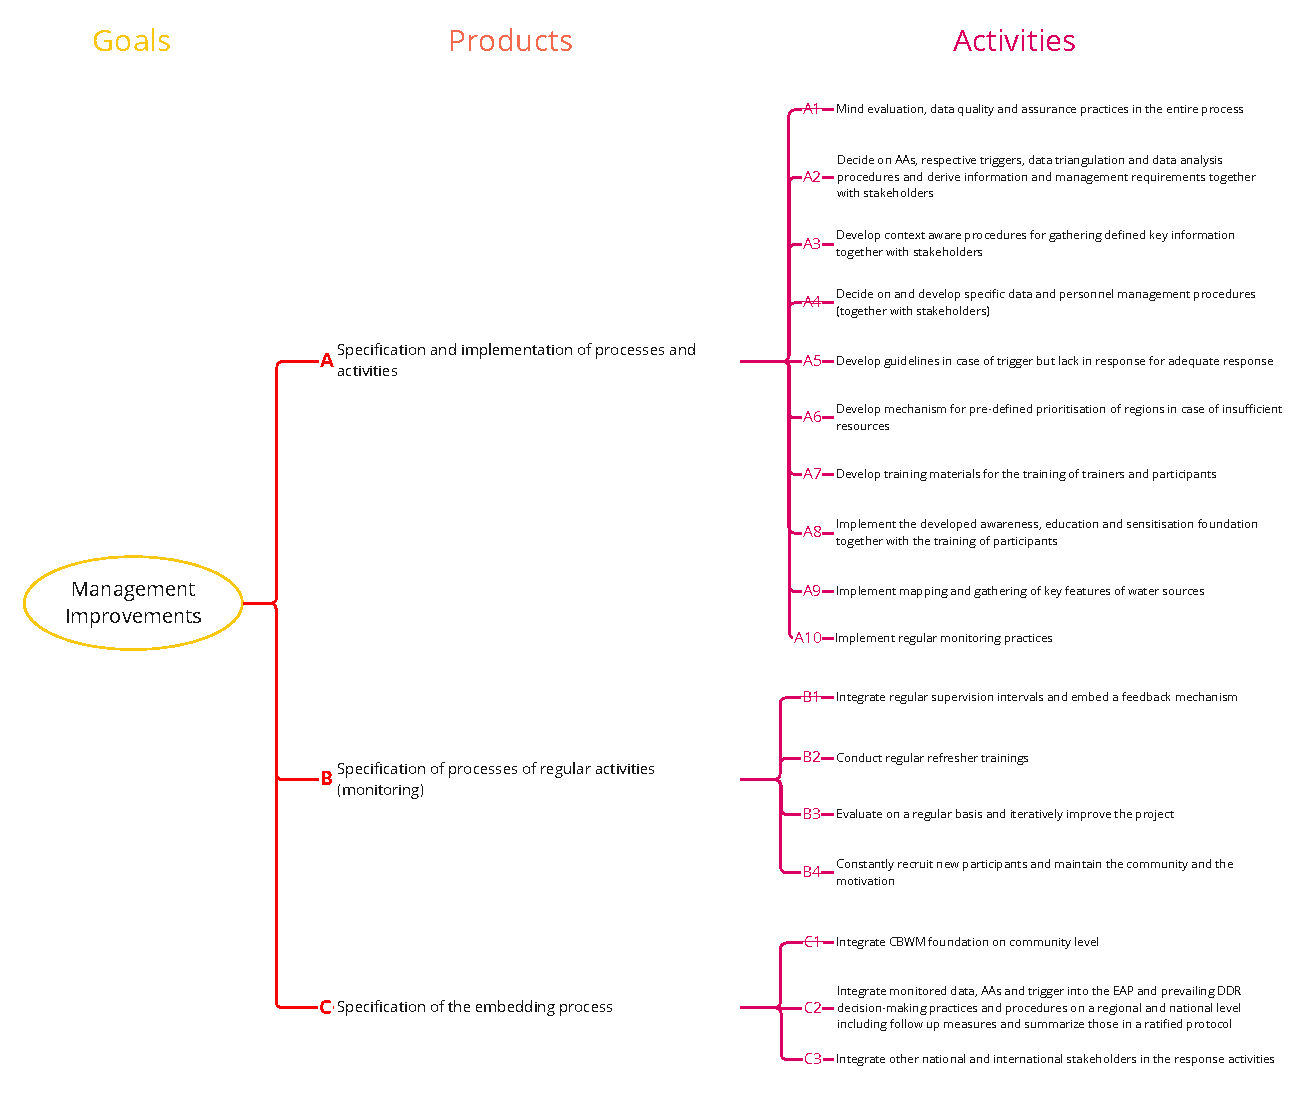
\includegraphics[width=1.0\textwidth]{figures/2023_MA_results_management.pdf}
    \decoRule
    \caption[The Management]{The Management. Source: Own representation.}
    \label{fig:res_management}
\end{figure}

\pagebreak


\section{Application: Focus Somaliland}\label{sec:f_a}
% FIXME: beim weiteren Überlesen: NYSS is now primarily in section subsubsec:cbs
In this part, by applying the roadmap and project requirements described above, the second research question of this thesis is tackled in order to ultimately achieve the overall aim of the research. Therefore, the results in this section are primarily geared towards identifying and implementing adequate water level monitoring of the water source type of berkads in order to trigger respective \acrlongpl{aa}. The third stage is structured following the project requirement catalogue. The Stages 4 to 6 refer their findings to the catalogue. However, because of their specific foci, they are not structured according to the catalogue. The above already displayed tree-diagrams can also additionally be found in the respective GitHub repository in Appendix \ref*{TODO:}. This provides the reader with a simultaneous reference option, as the products and activities will only be mentioned by their abbreviations and not by their full name, to enhance readability.

\subsection{Application Stage 1: Context \& Problem Identification}\label{subsec:stage1_appl}
%%%%%%%%%%%%%%%%%%%%%%%%%%%%%%%%%%%%%%%%%%%%%%%%%%%%%%%%%%%%%%%%%%%%%%%%%%%%%%%%%%%%%%%%%%%%%%%%%%%
%%%%%%%%%%%%%%%%%%%%%%%%%%%%%%%%%%%%%%%%%%%%%%%%%%%%%%%%%%%%%%%%%%%%%%%%%%%%%%%%%%%%%%%%%%%%%%%%%%%
%%%%%%%%%%%%%%%%%%%%%%%%%%%%%%%%%%%%%%% !!! SECTION 1 !!! %%%%%%%%%%%%%%%%%%%%%%%%%%%%%%%%%%%%%%%%%
%%%%%%%%%%%%%%%%%%%%%%%%%%%%%%%%%%%%%%%%%%%%%%%%%%%%%%%%%%%%%%%%%%%%%%%%%%%%%%%%%%%%%%%%%%%%%%%%%%%
%%%%%%%%%%%%%%%%%%%%%%%%%%%%%%%%%%%%%%%%%%%%%%%%%%%%%%%%%%%%%%%%%%%%%%%%%%%%%%%%%%%%%%%%%%%%%%%%%%%

The brief water source data analysis along with given context, resource restrictions, stakeholders and comparable projects as well as problem and goal statements of the interviewees are covered in this first stage. It also builds on the preceding case study area section \ref{sec:case_area} in chapter \ref{chapter2}.\newline
% current situation
The current drought and water scarcity situation in Somaliland has now lasted five years and has greatly impacted the water sector in Somaliland in terms of quantity and quality (I1). I1 describes the current crisis as \textit{"huge and response activities are being overwhelmed by the need"} which will lead to \textit{"commercialization and overpricing of fresh water"} further exacerbating the situation. This was underlined by I3 who describes the current water situation of the rural population as \textit{"whatever source of water they can find is what they have"}. I3 further mentions, that the people sometimes \textit{won't have enough water to wash their hands"} or for other necessary things and that \textit{"they [then] don't think of what kind of water they can get, whether it's bad or something like that"} but only focus on having at least something to drink. Increased water shortage because of bad quality was also reported in the literature (see section \ref*{subsec:water_quality}). Water can potentially be contaminated at all stages of the water collection process, from the initial abstraction of water, through transport and storage, to the use of the water (I3). Water quality is difficult to assess on site, as the the colour is not a good indicator and other parameters can only be determined technically which required equipment and training (I1, I3). Furthermore, I3 confirms the reports in literature that contamination of water in berkads, through their shared use with animals, can happen even before water withdrawal. This depends very much on the construction method and how it is used. The rehabilitation as well as training how to adequately use a berkad are already activities of the \acrshort*{srcs} (I3) and besides the water quality, the quantity also depends on the kind of construction and of withdrawal. According to I3, supply period can range from one month to half a year, so information on these parameters is crucial for estimating the potential duration of supply (I3).\newline
Water monitoring and management is not seen as a problem in urban areas as there is an agency responsible for water supply but the problem is primarily located in rural and nomad areas, where 70\,\% of the people live, according to I3. \autocite{republicofsomaliaCountryProfile20212021}, on the other hand, estimates an urban and semi-urban, sedentary population rate of 53\,\%.\newline
% problem
The selection of beneficiaries for response activities of the \acrshort*{srcs} are currently conducted on the basis of a preceding joint priority setting with the government. This prioritisation is based on \textit{"assumed vulnerability per community based on Number of \acrfull{idp} camps in the area, number of women headed families, predicted IPC classifications etc."} (I1.2). \acrlongpl{aa} have not been implemented due to the \textit{"already prevailing crisis"} where the \textit{"needs are [already] dire and the current \acrshort{srcs}'s focus is on response mechanisms to address the already visible impacts of drought"} (I1.2). Thus, the overall \textit{"end goal [of this project] will be to counter water shortages"} (I1) proactively but \textit{"there has been any actions yet due to the fact that there is no water monitoring and trigger mechanism in place"} (I1). The monitoring was itself hampered by the fact that \textit{"Berkads location data is currently missing"} (I1). This statement compares well with the experience of the current project team working on the EAP implementation and the assessment of available data sets (\acrshort{eap} project team, personal communication, 04.03.2022).\newline
Table \ref*{TODO} shows all available data sets of water sources in Somaliland, provided by \acrshort*{swalim}. % and OSM (?)
% ! noch mal die einzelnen Interviewees vorstellen.

\missingfigure{table swalim water sources} % see joplin
% maybe add OSM data as well.. quite some work though as not one single tag can be used.. could be a good comparison though. Only one data provider is a bit mehh.. and no OSM is hard to explain and I got the python scripts already.. need to refine the methodology though. Should be worth it. + add settlements to it
\begin{table}[!h]
    \caption[Water Sources]{All currently available data sets for water sources provided by SWALIM in Somaliland. Data Source: \autocite{swalimSomaliaWaterSources,swalmSomaliaWaterSources2023}}
    \begin{adjustbox}{center,max width=\linewidth}
        \def\arraystretch{1.5}
        \begin{tabular}{rlrrrrrrrr}
            \toprule
            \bf Year & \bf Name    & \bf Total & \bf Berkads & \bf Boreholes & \bf Dams & \bf Dug Wells & \bf Springs & Other \\
            \midrule
            2018 & Strategic WS    & 1792      & 50           & 357          & 319      & 853           & 163         & 50    \\
            2019 & Surface WS      & 1210      & ~            & 357          & ~        & 853           & ~           & ~     \\
            2020 & Strategic WS    & 3014      & 218          & 885          & 185      & 1422          & 245         & 59    \\
            2022 & Strategic WS    & 685       & ~            & 490          & 41       & 138           & 16          & ~     \\
            2023 & SWIMS Dashboard & 3648      & 217          & 1339         & 225      & 1547          & 261         & 59    \\
            \bottomrule
        \end{tabular}
    \end{adjustbox}
    \label{tab:res_data}
\end{table}

% data set
The spatial distribution of the datasets across Somalia is relatively balanced, with focal points in the regions with many or larger settlements. Based on the \acrshort{swalim} settlement data set, there are currently 2123 settlements in Somaliland. These settlement data are mostly from the years 2002 and 2006. The total number of water sources varies greatly between all datasets. The timeliness of the data also has a wide range, from relatively few pieces of data from 2019 in the 2020 dataset to data from the 1980s in the same dataset is much represented. The 2022 dataset misses information about timeliness altogether and the other datasets all have many blank entries as well. Furthermore, many water sources are labelled as 'abandoned' or 'non-functional', e.g. in the 2022 dataset those are 147 out of 685.\newline
% stakeholders
The data sets are fed by many sources and actors e.g. FAOSWALIM or other UN organisation, \acrshort*{mowr}, \acrshort*{nadfor} and other NGOs which constructed some water sources in some communities (I1). These actors, along with the community and their elders, local government representatives, SRCS and their volunteers and private berkad owners are also the potential stakeholders of the mapping and monitoring of berkads. Here, I1 notes, that besides the \acrshort*{srcs}, the \acrshort*{mowr}, \acrshort*{nadfor} and the constructing NGOs are the most important stakeholders. The \acrshort*{mowr} and NGOs have the technical expertise in construction, rehabilitation and monitoring and \acrshort*{nadfor} has a comparable community level programme for monitoring \textit{"livestock body condition, market prices as well as weather variables"} (I1).\newline
% comparable projects
Other comparable programmes exist from \acrshort*{ocha}, \acrshort*{brcis} and the \acrshort*{cbs} programme run by the Ministry of Health, the \acrshort{srcs} and the \acrshort*{nrc}. While these projects may broadly be comparable in terms of focus on \acrshortpl{aa}, none of the Interviewees know of a project that conducts similar things to this works aim (I1, I2, I3). I2 also suggests that the projects are close enough to each other to pass on experiences and recommendations, e.g. from the \acrshort{moh} to the \acrshort{mowr}, in order to overcome initial scepticism and reluctance.\newline
% challenges, limitations, requirements
Challenges, limitations and requirements are mentioned in areas of privately owned berkads, community expectation handling and the dissolution of misconceptions as well as potentially already overstretched SRCS staff and volunteers (I1). I1 mentioned, that private owners of berkads may prevent the volunteer from gaining access to their berkad which would result in less information on the one hand but also in tension in the community on the other. Giving information from the community to someone else may also generally require some explanation (I2). Furthermore, some \textit{"information on past details per particular geographical areas"} (I1.2) can be difficult to access, as \textit{"Somalis are highly mobile communities"} (I1.2). The monitoring could furthermore develop \textit{"hugh expectations from the communities as there is the ongoing drought. Whenever there is monitoring of resources, communities believe this should be followed up by instant aid"} (I1).\newline
% potential solutions
Addressing some of the challenges mentioned above, the \textit{"community elders should be engaged before the start of the mapping and monitoring as they will help dispel misconceptions about the project"} (I1) and the \textit{"ministry of water resources should be in the loop during the entire project duration"} (I1). Nonetheless, the \textit{"community and SRCS goals match as both focus on closing the knowledge [gap] currently existing"} (I1) in regard to the number, status of ownership, location and capacity of the berkads per community, district and regional level. This will \textit{"inform decision-makers on the priority areas to focus on"} (I1). Therefore, I1 expects that this information from the site triangulated with weather forecasts can help to form robust triggers to take appropriate and informed \acrlongpl{aa} before critical water levels are reached.

\subsection{Application Stage 2: Feasibility Assessment}\label{subsec:stage2_appl}
%%%%%%%%%%%%%%%%%%%%%%%%%%%%%%%%%%%%%%%%%%%%%%%%%%%%%%%%%%%%%%%%%%%%%%%%%%%%%%%%%%%%%%%%%%%%%%%%%%%
%%%%%%%%%%%%%%%%%%%%%%%%%%%%%%%%%%%%%%%%%%%%%%%%%%%%%%%%%%%%%%%%%%%%%%%%%%%%%%%%%%%%%%%%%%%%%%%%%%%
%%%%%%%%%%%%%%%%%%%%%%%%%%%%%%%%%%%%%%% !!! SECTION 2 !!! %%%%%%%%%%%%%%%%%%%%%%%%%%%%%%%%%%%%%%%%%
%%%%%%%%%%%%%%%%%%%%%%%%%%%%%%%%%%%%%%%%%%%%%%%%%%%%%%%%%%%%%%%%%%%%%%%%%%%%%%%%%%%%%%%%%%%%%%%%%%%
%%%%%%%%%%%%%%%%%%%%%%%%%%%%%%%%%%%%%%%%%%%%%%%%%%%%%%%%%%%%%%%%%%%%%%%%%%%%%%%%%%%%%%%%%%%%%%%%%%%

In this stage, the practical capacities, and applicability and suitability of the \acrshort*{cbm} and \acrshort*{mcs} approach for community-based water monitoring were examined in this context. The SRCS has 249 paid employees, of which 30 work in the risk management and \acrlong*{aa} domain and an additional 1500 volunteers are "evenly spread" across the country (I1). I3 emphasises the \textit{"good relations and good reputation"} that \acrshort*{srcs} has within the communities, making them \textit{"one of the most trusted organizations in the country"} which helps to do programs at community level. The 'feasibility study on Potential Use of \acrshort*{fbf} for SRCS' \autocite[44]{scrsFeasibilityStudyPotential2022} recognizes a \textit{strong national organization} with a \textit{strong volunteer base at community level} that \textit{provides monitoring and hazard warning capacities}. Furthermore, \textit{highly skilled and experienced management staff at coordination and Branch levels} is stated. Nonetheless, \textit{minimal domestic resource mobilization} and a \textit{lack of meteorological, geo-spatial analysis, data management and IT staff} has also been detected.\newline
% NYSS
This lack of resources and digital capacities was addressed in the \acrshort*{cbs} project by the \acrshort*{nrc} and their NYSS platform. Generally, \acrshort{cbs} is \textit{nothing new in itself and often used in health contexts} (I2). \acrshort*{cbs} in Somaliland started in Burao in 2018 with 75 community volunteers, as cholera had broken out in the same region in 2017 (I3). After the pilot was successful, \acrshort*{cbs} has since been extended to all regions but \textit{\acrshort*{srcs} only focusses on hot spot areas where they expect outbreaks to happen} (I3). This development took place over the course of a year with much feedback from the \acrshort{srcs} and NYSS is now \textit{"very effective and very supportive"} (I3). The \acrfull*{moh} was and is \textit{constantly in the loop to decide together what, how, when and who} and could gain good experiences with NYSS over the years (I2). By now, NYSS is well embedded in the local conditions and \textit{"mobile teams [...] can be deployed immediately within hours so they can do the response"} (I3) in collaboration with other partners such as the \textit{"government, \acrshort{moh}, \acrshort{who}, and other sister \acrshort{rcrc} organisations} (I3).\newline
% reasoning why this approach works
I2 mentions, that the monitoring of water sources \textit{would fit well thematically, because it [low water levels and poor water quality] is a health risk} and that although it would require some adjustments and considerations, it would organically expand technical expertise and functionality as it is not \textit{radically new}. Besides NYSS, being methodologically similar but different in thematic orientation, several other projects could be identified in literature, that are oriented towards the same topic but differ in their implementation and operation procedures (compare section \ref*{subsubsec:cbwm}). It can be deduced from this that \acrshort{cbm} and \acrshort{mcs} can in principle be applied to the thematic issue. Furthermore, \autocite{fraislCitizenScienceEnvironmental2022} themselves describe approaches that focus on the "in situ monitoring" of water resources and at the same time benefit the respective participant as adequate for the use of a \acrlong{cs} approach. \acrshort{srcs} does not pay their volunteers but provides training and covers travel expenses as incentives. Moreover, volunteers are generally well regarded and are selected by the community itself. Intrinsic motivation is therefore present (I2, I3).\newline
\autocite{fraislCitizenScienceEnvironmental2022} prerequisites are thus fulfilled, and the key objectives of the \acrshort{rcrc}'s \acrshort{cbs} preliminary assessment can be answered positively. The task is applicable within a \acrshort{cs} approach and the \acrshort{srcs} is an adequate partner with sufficient capacities and experiences to implement the mapping and monitoring approach. The project can thus be further developed in Stage 3.

\subsection{Application Stage 3: Structure \& Design}\label{subsec:stage3_appl}
%%%%%%%%%%%%%%%%%%%%%%%%%%%%%%%%%%%%%%%%%%%%%%%%%%%%%%%%%%%%%%%%%%%%%%%%%%%%%%%%%%%%%%%%%%%%%%%%%%%
%%%%%%%%%%%%%%%%%%%%%%%%%%%%%%%%%%%%%%%%%%%%%%%%%%%%%%%%%%%%%%%%%%%%%%%%%%%%%%%%%%%%%%%%%%%%%%%%%%%
%%%%%%%%%%%%%%%%%%%%%%%%%%%%%%%%%%%%%%% !!! SECTION 3 !!! %%%%%%%%%%%%%%%%%%%%%%%%%%%%%%%%%%%%%%%%%
%%%%%%%%%%%%%%%%%%%%%%%%%%%%%%%%%%%%%%%%%%%%%%%%%%%%%%%%%%%%%%%%%%%%%%%%%%%%%%%%%%%%%%%%%%%%%%%%%%%
%%%%%%%%%%%%%%%%%%%%%%%%%%%%%%%%%%%%%%%%%%%%%%%%%%%%%%%%%%%%%%%%%%%%%%%%%%%%%%%%%%%%%%%%%%%%%%%%%%%

This stage is grouped into the four project requirement groups and lays the structure for the coming stages. The overall project aim to counter water shortages proactively is majorly hampered by missing information about the water source type berkad. Therefore, up-to-date information on water sources in Somaliland is needed. In particular, there is a lack of information on the important Berkad water sources (compare stage \ref*{subsec:stage1_appl}). Therefore, the focus of this project will be on gathering information about this specific water source type (I1). See chapter \ref*{subsec:water_sources} for further information about this water source type. I1 also named and chronologically ordered the most important fields of action that need to be realised in order to achieve this goal:

\begin{enumerate}
    \item Volunteer briefing and training
    \item Community sensitization
    \item Locating and gathering key information about berkads
    \item Determining respective \acrlongpl{aa} (own addition)
    \item Determination of the water level thresholds 
    \item Monitoring of the water level
    \item Triggering \acrshortpl{aa} based on pre-defined threshold 
\end{enumerate}

I1 highlights the importance of the actions 2, 3 and 7 as critical for the overall success of the project. For the design stage, I1 emphasises the determination of the threshold, \acrlongpl{aa} and respective trigger. As I1 draws his judgement from his work as the local program manager and coordinator, this project followed these priorities during the design process. This process is grouped by the project requirement catalogue in the following. The structure of each group follows the order of the products and respective activities, emphasis was given to the activities which contribute directly to the above mentioned priorities. To minimise repetition in the scope of this work, already covered areas are only referred to and not again outlined in detail. 

\subsubsection*{The Assemblage: Knowledge Building}\label{subsubsec:assemblage}

The majority of the activities of product (A) were already covered by previous stages and chapters. (A1) was extensively outlined in section \ref*{sec:fundamental_concepts}. (A2) and (A3) were covered by Stage 1 \ref*{subsec:stage1_appl}, \ref*{subsec:stage2_appl} and section \ref*{sec:case_area}. (A4) on the one hand will influence decision-making in the \acrshort{srcs} but further integration into e.g. governmental procedures could not be covered by this work. Activities A5 and A6 could also only be touched upon, but especially the topic of integration of local knowledge holds a lot of potential (see \ref*{subsec:indicators}).\newline
Product (B) could partly be covered by stage 2 \ref*{subsec:stage2_appl}. Results so far suggest that the network and individual volunteers are adequately trained, motivated and managed for the monitoring task, which laid the basis for Stage 4. In terms of adequate data management (C), feasible technical solutions could be identified from other projects and their practical applicability was demonstrated by the successful \acrshort{cbs} program of the \acrshort{srcs} (C1). Further exploration in Stage 5 was thus possible. (D) current evaluation and improvement procedures could be identified and are further described in Stage 6.\newline
(E1) initially important information about each berkad is summarized in figure \ref*{TODO:}. This compilation is based on section \ref*{subsec:water_sources}, and knowledge of I1, I2, and I3. The left, bold side are the information highlighted by the interviewees and summarize the key information. The right side displays information, that may be nice to know for further analysis, but is not regarded as critical for this project.

\begin{figure}[!htp]
    \centering
    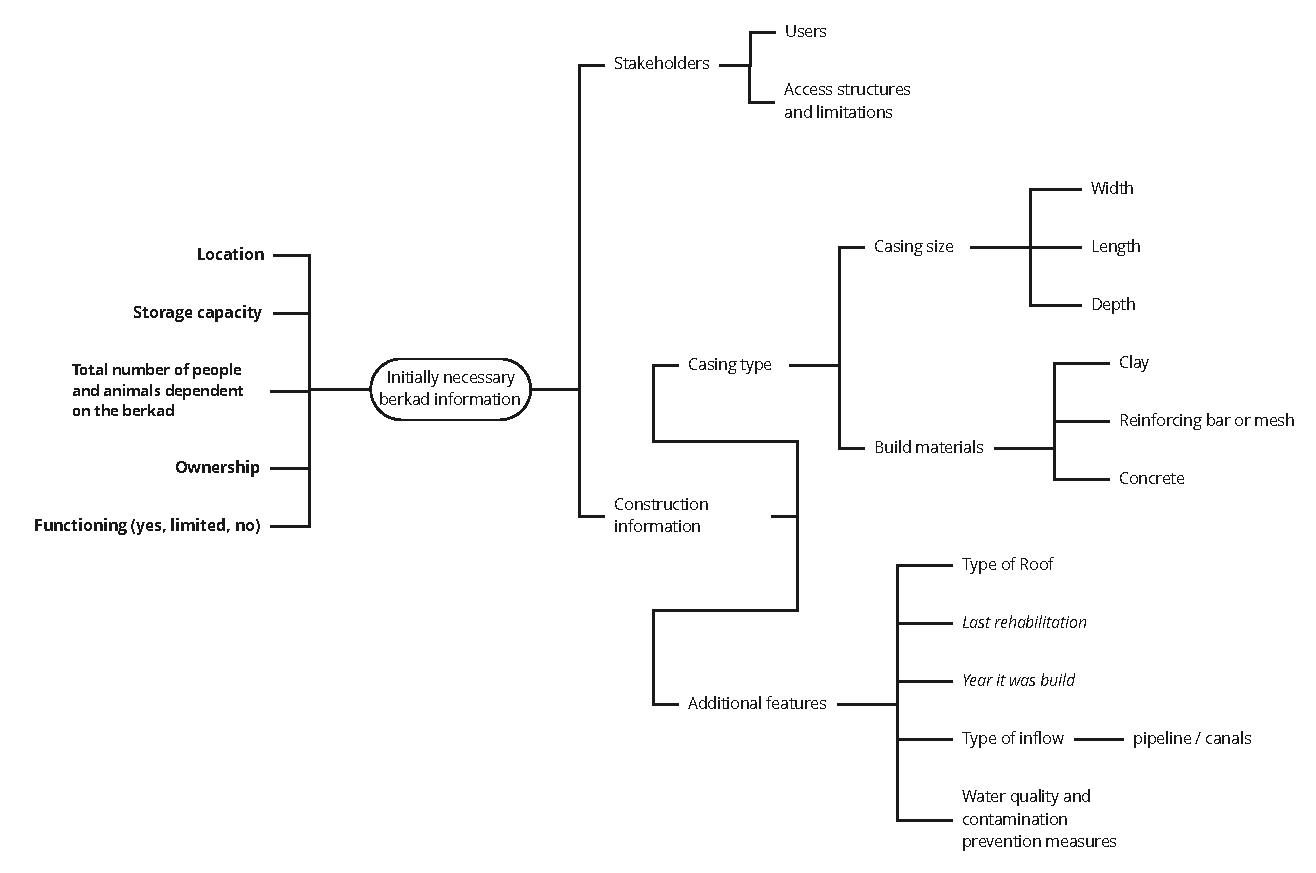
\includegraphics[width=1.0\textwidth]{figures/2023_MA_results_berkad.pdf}
    \decoRule
    \caption[Key Features of a Berkad]{Key Features of a Berkad. Source: Own representation.}
    \label{fig:res_berkad}
\end{figure}

In terms of (E2), location, storage capacity and construction information need to be identified initially and might need to be updated when e.g. the berkad is rehabilitated. These information will be gathered by \acrshort{srcs} professionals and therefore does not need to be included in the regular monitoring routine. (E2) a report about the condition of the berkad may only be necessary once a year (I1.2) while the number of people and animals may need a weekly or monthly reporting interval, depending on the fluctuation strength (I1.2). This information should be kept comparatively up to date, as the high mobility of Somalis means that this number can change relatively regularly and has a great influence on the amount of water abstraction (I1.2).\newline
(F1) the water level of the berkad was named as constantly changing indicator which should be monitored in a weekly interval (I1.2). The realisability and adequacy of this reporting frequency was also supported by I2 (F2). (F3) The data sets for the data triangulation are adopted from the overarching \acrshort{eap} and have not yet been determined at the time of writing.\newline 
Potential AAs that can be triggered in correspondence with a the surveyed information and certain water level threshold are listed below (G). 

\begin{itemize}
    \item Informing about water rationalisation and saving opportunities
    \item Information dissemination of climate and weather forecasts
    \item Distribution of drought-resistant crops
    \item Rehabilitation of berkads before the rainy season 
    \item Compensate private berkad owners to access their water
    \item Timely distribution of cash to enable communities to buy and stock fresh water
    \item Timely distribution of water purification tablets 
    \item Water trucking
\end{itemize}

Raising awareness and information dissemination need to be the foundation of this (see Groundwork \ref*{TODO:}, I1.2). The distribution of drought-resistant crops and other agricultural related actions need to be coordinated with the \acrfull{moad}. The rehabilitation of berkads before the rainy season needs to be related to seasonal triggers as this actions will help to store available rain water and won't directly help in times of acute water shortages. I1.2 notes, that the involvement of private berkad owners \textit{"could be limited as they are more concerned about their business models i.e selling of the water and preserving their berkads than being part of the overall response/Anticipatory Action mechanism"}. Nevertheless, I1.2 sees potential in working with private berkad owners and suggests e.g. the rehabilitation of their berkads \textit{"in return for their involvement in response and Anticipatory Action activities"} as viable \acrshort{aa}. The distribution of cash is a widely applied \acrshort{aa} in \acrshort{fbf} projects and can help in many cases. Distribution of water vouchers is an alternative to direct cash and has already been used successfully in Somaliland (see section \ref*{subsec:case_eap}). Water purification tables and information for waterborne disease prevention are already disseminated by the \acrshort{srcs} volunteers together with hygiene and health promotion activities but could be better targeted by more timely and localised information (I3). The required lead time, tangible and intangible resources, information requirements and involved roles (G2 \& G3) of these \acrshortpl{aa} are illustrated in figure \ref*{fig:res_aa}. 

\begin{figure}[!htp]
    \centering
    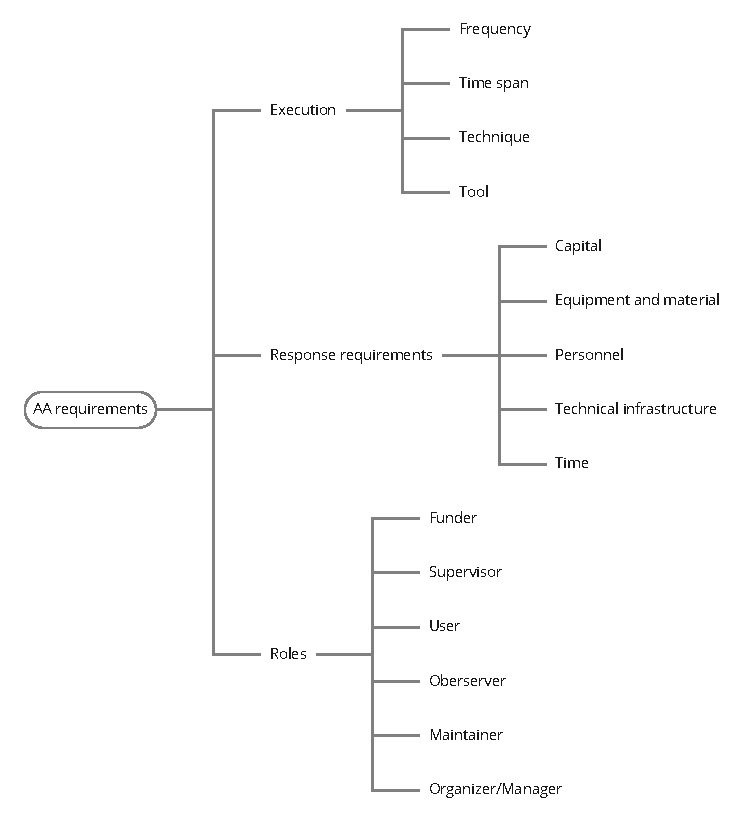
\includegraphics[width=1.0\textwidth]{figures/2023_MA_results_AA.pdf}
    \decoRule
    \caption[Requirements for Anticipatory Actions]{Requirements for Anticipatory Actions. Source: Own representation.}
    \label{fig:res_aa}
\end{figure}

This list is not comprehensive and needs to be refined for each \acrshort{aa}, which is illustrated in figure \ref*{fig:res_water_truck} for the \acrshort{aa} \textit{water trucking}.

\begin{figure}[!htp]
    \centering
    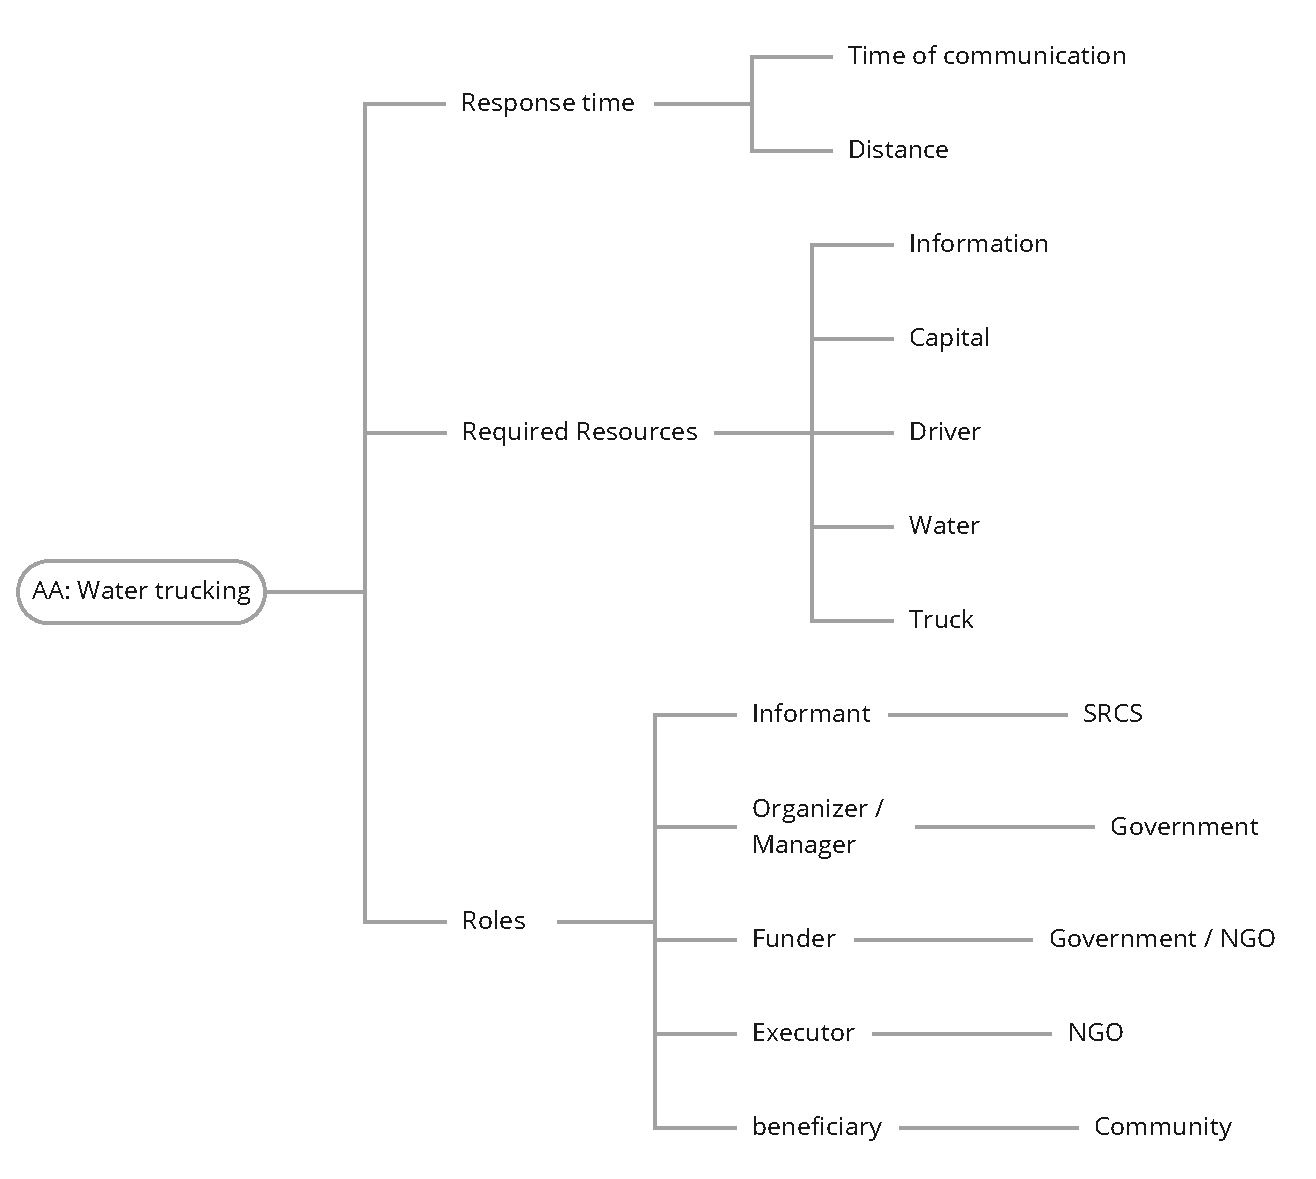
\includegraphics[width=1.0\textwidth]{figures/2023_MA_results_trucking.pdf}
    \decoRule
    \caption[Water Trucking parameters]{Important Information about the Anticipatory Action of water trucking. Source: Own representation.}
    \label{fig:res_water_truck}
\end{figure}


Water trucking is a common measure to cope with acute water shortage in Somaliland (I1.2, I2). Information for water water trucking comes, thus far, from \acrshort{srcs} assessments, from the community themselves, government agencies, \acrshort{fsnau} or other NGOs (I3). This type of information transmission can be timely and may be incomplete. The water transport itself can take a long time and can be relatively expensive due to the distance and high demand (I1, I3). It is financed by various stakeholders, including the community themselves and private donors (I3). Self-financed water trucking is especially common in the beginning of the initial phase of drought but if the people cannot afford to buy water any more and their livestock becomes weak or dies, \textit{"[...] this is the time they talk to the other NGOs or the government and say we need support [...]"} (I3). Currently, the following prioritisation of water trucking by the regional and national stakeholders is primarily based on government decisions and focusses on the most vulnerable communities (I3). This decision-making process could not be explained in more detail by (I3) other than it is a \textit{joint effort by all stakeholders}. The \acrshort{srcs} does not truck water themselves (I1.2).\newline
(H1) potential water level thresholds were suggested by I1.
\begin{itemize}
    \item Empty (no water at all)
    \item Critical (1 day of water supply remaining)
    \item Low (3 days of water supply remaining)
    \item Middle (5 days of water supply remaining)
    \item High (full capacity)
\end{itemize}
I1 further specified the \textit{Low} category to trigger the \acrshort{aa} of \textit{water trucking} (H2). These water levels either require local knowledge about how long the water will last or require the analysis of the exact or categorized water level with the known berkads capacity. The first option would outsource the triangulation of available resources and amount abstraction to the communities predictions. I1.2 notes, that \textit{"these kinds of predictions are good as communities usually have their own control measures to ensure equitable distribution of water e.g. how many containers per family etc. The berkads are usually locked to ensure there is controlled access to the water stored"}. The second requires good information about the berkad itself and a feasible method to interpolate this with the regularly measured information. \autocite{gualazziniEWEAEarlyWarning2021} however, proposed more seasonal focussed threshold levels for berkads (see chapter \ref*{subsec:case_eap}). (H3) the short-term thresholds may be feasible to short-term and fast \acrshortpl{aa}, whereas seasonal information may trigger \acrshortpl{aa} such as the rehabilitation of berkads and information campaigns.

\subsubsection*{The Groundwork: Laying the foundation}\label{subsubsec:groundwork_appl}

Volunteer briefing and training together with following sensitization of the community are the first two measures that lay the foundation for the implementation of this project (see \ref*{subsec:stage3_appl}, I1). (A1) major challenges could be identified in community expectation handling and the involvement of private berkad owners (I1, I2). I1 suggested, the early engagement of community elders to address community internal issues and the continuous involvement of the \acrshort{mowr} for organisational and stakeholder management. Awareness-raising activities and dissemination of information may include knowledge of water quality improvement techniques, water conservation strategies, early warnings and a detailed explanation of the reasons for regular water level reporting before the start of the project (I1, I2). It also needs to be \textit{communicated, discussed and decided beforehand},  what happens in cases when thresholds are reached but no response is possible (I2). \textit{Otherwise, it could fall back negatively on the SRCS and the Volunteer} (I2). Furthermore, I1.2 highlights the importance, to establish \textit{"a robust feedback and complaints mechanism that ensures communities can easily relay their feedback.} right from the start. The development and implementation of products (A2), (B), (C), (D), and (E) must happen in close collaboration with local stakeholders and were thus out of scope of this work. Nonetheless, the work with the community should be fruitful as their goal to \textit{"ascertain whether these water bodies are able to withstand the demand during drought periods"} overlap with the project goals (I1).\newline
The integration of the light \acrshort{iwrm} framework developed by \autocite{dayCommunitybasedWaterResources2009} was presented in section \ref*{subsubsec:cbwm} and needs to be further discussed with local stakeholders and interrelated with prevailing procedures.

% to facilitate this and further implement this roadmap --> policy (social frameworks) and methods (practical techniques and tools) need to be developed.

% As with most activities, that need close collaboration on site, this was out of scope of this study.

% \subsubsection*{Integrated Water Management (Goal and Groundwork for mapping/monitoring)}

% ground work -> public education --> inform community about water shortages (?) -> create "agreement on water priorization during times of acute drought" + "a common shared agreement to prevent water resource contamination, as well as mitigating over-abstraction." (Day, 2009: 52)

% BUT:
% “Communities may not always represent a homogeneous, consenting group” ([Day, 2009, p. 52](zotero://select/groups/4773535/items/YWSNQ8A2)) ([pdf](zotero://open-pdf/groups/4773535/items/ETPCI5RI?page=7&annotation=NMA3CWDS))
% --> different interests, resources, knowledge, access rights, own hierarchy + status level

% how about private water sources?
% “Strikingly, the traditional influence of sheikhs in water management does not, however, extend to supervision of private wells or boreholes operated by farmers or individual landowners. Sh” ([Day, 2009, p. 55](zotero://select/groups/4773535/items/YWSNQ8A2)) ([pdf](zotero://open-pdf/groups/4773535/items/ETPCI5RI?page=10&annotation=FXZW8RBU))

% AA -> manage water and prioritize effectively (e.g. start with it now)
% “This is significant because in drought-prone environments little at tempt is made to inform communities about their available ground water resources and there is minimal emphasis or preparation for monitoring groundwater fluctuations, prioritizing water usage dur ing periods of hardship or assisting communities to develop basic contingency plans with relief agencies or local authorities acting as a back-stop to provide support during periods of acute” ([Day, 2009, p. 51](zotero://select/groups/4773535/items/YWSNQ8A2)) ([pdf](zotero://open-pdf/groups/4773535/items/ETPCI5RI?page=6&annotation=6C4BAHSE))

% “hardship. When describing community water projects, 'sustainability' is often referred to. In reality the immediate challenge is to introduce sound steward ship of water resources to assist communities to resist and recover from drought or low and variable rainfall” ([Day, 2009, p. 51](zotero://select/groups/4773535/items/YWSNQ8A2)) ([pdf](zotero://open-pdf/groups/4773535/items/ETPCI5RI?page=6&annotation=DA9BJCDN))

% “r of distinct advantages of engaging in commu nity-based water resource mana” ([Day, 2009, p. 51](zotero://select/groups/4773535/items/YWSNQ8A2)) ([pdf](zotero://open-pdf/groups/4773535/items/ETPCI5RI?page=6&annotation=85TSGZK9))

% FIGURE of the framework: “Figure 2. Community-based water resource manageme” ([Day, 2009, p. 59](zotero://select/groups/4773535/items/YWSNQ8A2)) ([pdf](zotero://open-pdf/groups/4773535/items/ETPCI5RI?page=14&annotation=BAMSY255))
% %% --> this framework as 'base'/foundation/Early Action/AA?

% “Local water users often possess detailed indigenous knowledge related to water resources, water needs and historical change that has occurred related to water use. 
% Water users recognize that water is a fundamental component of their subsistence-based livelihoods, which helps to weave rela tionships between water users. 
% Communities are able to monitor agreed water usage on a daily basis, as part of their daily activities. 
% Communities often have historical mechanisms for conflict and dispute resolution related to water resource management, which may require continued support and assistance to evolve and adapt to global challenges. 
% Effective water management requires community participation; this principle is well understood in development li” ([Day, 2009, p. 52](zotero://select/groups/4773535/items/YWSNQ8A2)) ([pdf](zotero://open-pdf/groups/4773535/items/ETPCI5RI?page=7&annotation=4RVGKM5R))

% “However, responsible planning for drought mitigation at community level is often omitted.” ([Day, 2009, p. 47](zotero://select/groups/4773535/items/YWSNQ8A2)) ([pdf](zotero://open-pdf/groups/4773535/items/ETPCI5RI?page=2&annotation=S4ACQRPL))

% “Communities frequently remain excluded from any basic capacity building, centred on water resource management, as part of a localized Integrated Water Resources Management (IWRM) programme.” ([Day, 2009, p. 47](zotero://select/groups/4773535/items/YWSNQ8A2)) ([pdf](zotero://open-pdf/groups/4773535/items/ETPCI5RI?page=2&annotation=WBL45NKR))

% “Community-based water resources management” ([Day, 2009, p. 47](zotero://select/groups/4773535/items/YWSNQ8A2)) ([pdf](zotero://open-pdf/groups/4773535/items/ETPCI5RI?page=2&annotation=RQLJMKL7))

\subsubsection*{The Innovations: Developments and Improvements}\label{subsubsec:innovations_appl}

Besides the identification of a way to integrate \acrshort{iwrm} practices into local procedures and structures, more technical solutions were also required to be developed or adapted. (A1) important primary information about the water source berkad could be identified by the method of expert interviews. (B1) and (C1) could be identified through interviews and literature analysis, where (B1) will either be a kind of categorised yardstick or a local estimation based on experience or a combination of both. However, a thorough assessment and subsequent adjustment of the practical suitability will only be possible in a pilot study. This is especially true for their evaluation (A2) and (B1). Several data management methods could be identified in literature, see sections \ref*{subsec:mcs} and \ref{subsec:case_eap}, and applied in practice by other projects see sections \ref*{subsubsec:cbs} and \ref*{subsubsec:cbwm}. The desk-based evaluation (D1) has shown advantages and disadvantages for all potential methods, from simple to very dedicated implementations, thus allowing an informed decision in the coming chapter. Building on this, a first draft of possible SMS codes could be developed for (1) a data based application and (2) a more local knowledge based version:

\begin{center}
    \begin{minipage}{0.9\textwidth}
        \begin{align*}
            1.\: Weekly:\ &\#\: Water\: Source\: ID\: \#\: Water\: Level\: \#\: Functioning/Accessible\\
            2.\: Weekly:\ &\#\: Water\: Source\: ID\: \#\: Predicted\: Supply\: Duration\: \#\: Functioning/Accessible\\
            \\
            1.\: Monthly:\ &\#\#\: Water\: Source\: ID\: \#\: Number\: of\: dependent\: people\: \#\: Number\: of\: dependent\: animals\\
            2.\: Monthly:\ &\#\#\: Water\: Source\: ID\: \#\: Daily\: Amount\: of\: Withdrawal\\
            \\
            1.\: Annually:\ &\#\#\#\: Water\: Source\: ID\: \#\: Water\: Source\: Condition\\
            2.\: Annually:\ &\#\#\#\: Water\: Source\: ID\: \#\: Water\: Source\: Condition\\
        \end{align*}
    \end{minipage}
\end{center}

Hereby, the different report types are marked with the different number of starting '\#'. The \textit{Water Source ID} may be a composite of regional, district, and community identifiers along with a specific water source number. The \textit{Water Level} or \textit{Predicted Supply Duration} refers to the amount of water that is still available and the \textit{Functioning/Accessible} code may indicate if the source is functioning and/or accessible to the community. These two indicators could be combined in one number, as there are only four possible combination possibilities. With this, social and technical aspects could be monitored. The monthly codes relate to the amount of withdrawal and thus takes account of potentially changing demand conditions. The \textit{Water Source Condition} is difficult to limit on one number and more might be necessary as there are many different factors that can influence the condition (see figure \ref{TODO: List of initially necessary berkad information}). The number of codes is deliberately confined by a maximum of three codes, as this was the recommendation and limitation by I2 (see Stage 5, section\ref{subsec:stage5_appl}). The codes may only be seen as recommendations and will need to be evaluated and adapted in the future work.

\subsubsection*{The Management: Mapping \& Monitoring}

This last group of the project requirement catalogue comprises activities for evaluation and decision-making on the pre-identified conditions in the preceding sections. Though, due to the overarching ongoing \acrshort{eap} development and no possibility to conduct studies on site, no decision or on site evaluation could be made in the context of this work. Nevertheless, a lot of information and good practice could be gathered and organised appropriately in the presented groups in the previous phases which will greatly facilitate future evaluation and decision-making.\newline


%%%%%%%%%%%%%%%%%%%%%%%%%%%%%%%%%%%%%%%%%%%%%%%%%%%%%%%%%%%%%%%%%%%%%%%%%%%%%%%%%%%%%%%%%%%%%%%%%%%
%%%%%%%%%%%%%%%%%%%%%%%%%%%%%%%%%%%%%%%%%%%%%%%%%%%%%%%%%%%%%%%%%%%%%%%%%%%%%%%%%%%%%%%%%%%%%%%%%%%
%%%%%%%%%%%%%%%%%%%%%%%%%%%%%%%%%%%%% !!! COMMUNITY BUILDING !!! %%%%%%%%%%%%%%%%%%%%%%%%%%%%%%%%%%
%%%%%%%%%%%%%%%%%%%%%%%%%%%%%%%%%%%%%%%%%%%%%%%%%%%%%%%%%%%%%%%%%%%%%%%%%%%%%%%%%%%%%%%%%%%%%%%%%%%
%%%%%%%%%%%%%%%%%%%%%%%%%%%%%%%%%%%%%%%%%%%%%%%%%%%%%%%%%%%%%%%%%%%%%%%%%%%%%%%%%%%%%%%%%%%%%%%%%%%

\subsection{Application Stage 4: Community \& Stakeholder}\label{subsec:stage4_appl} % volunteers + SRCS + training - etc.

In the context of this project, the community volunteers of the \acrshort{srcs} are the contributing participants. The findings of this section contributed to the knowledge base primarily in areas (A4) to (A6) and (B) and form the basis for the participant and community related products and activities of the \textit{Groundwork} and \textit{Management} group. The volunteers are commonly not recruited by the \acrshort{srcs} in the common sense but rather chosen by the community (I3). Therefore, they are usually not primarily selected on the basis of their education or skills, but on the basis of the community's own criteria (I3). The decision on who becomes a volunteer is generally made by the community committee and their elders (I2). I3 notes that volunteers generally have a \textit{"good reputation in the community"}. \textit{"After the selection, SRCS is doing a small assessment about e.g. reading and writing skills and then provide training to them"} explained I3 in regard to the volunteers. Besides the social prestige, this training is also the primary extrinsic incentive to become a volunteer as the volunteers are not compensated otherwise (I2). Thus, volunteers need to be intrinsically motivated and \textit{"willing to be a volunteer"} (I3). After the training, the volunteers are send back to their communities and start working there (I3). Volunteers are \textit{mostly women as they stay in the community and do not travel as much as men} (I2). The work includes raising awareness about health and prevention hazards and informing about mitigation measures, as well as directly responding to them and, in the context of \acrshort{cbs}, reporting (I3). Currently, in case of water shortage, volunteers educate people on how to prevent waterborne diseases by providing hygiene and health education and distributing water purification tablets. (I3).\newline
Preliminary trainings, supervision and regular refreshers were seen, especially in the beginning, as important and as a great success factor by I2 and I3. In the \acrshort{cbs} program, refreshers were conducted in a monthly interval but this is no longer necessary in that frequency as the \textit{volunteers know their business by now} (I2). Nonetheless, supervisors still validate and clarify reports, e.g. via phone or on-site visits. As already described in Stage 2 (section \ref*{subsec:stage2_appl}), \acrshort{srcs} spends a lot of time on community bond building and thus generally has a very good reputation with the communities (I2, I3). This greatly facilitates the information flow and response together with other stakeholders such as the \acrshort{moh} or NGOs (I2).\newline
A selection of other national and international stakeholders were already mentioned in section \ref{subsec:case_eap}. The Interviewees often mentioned the importance of the \acrshort{mowr} and their early involvement. I2 mentioned, that they had many discussions with the \acrshort{moh} when integrating the \acrshort{cbs} project and that these discussions are still ongoing. However, I2 also mentions, that in their recent evaluation, \textit{the confidence in the \acrshort{moh} is not so great}. \textit{Many organisations come to the MoH with their own instruments, methods and goals} which can complicate the integration of projects and increases the competition. Therefore, I2 started to work with lower agencies instead but highlighted, that for the case of \acrshort{cbs}, experiences might be transferable from the \acrshort{moh} to the \acrshort{mowr}. 
% TODO: noch mal den Absatz überlesen. Da war ich müde..

%%%%%%%%%%%%%%%%%%%%%%%%%%%%%%%%%%%%%%%%%%%%%%%%%%%%%%%%%%%%%%%%%%%%%%%%%%%%%%%%%%%%%%%%%%%%%%%%%%%
%%%%%%%%%%%%%%%%%%%%%%%%%%%%%%%%%%%%%%%%%%%%%%%%%%%%%%%%%%%%%%%%%%%%%%%%%%%%%%%%%%%%%%%%%%%%%%%%%%%
%%%%%%%%%%%%%%%%%%%%%%%%%%%%%%%%%%%%% !!! DATA MANAGEMENT !!! %%%%%%%%%%%%%%%%%%%%%%%%%%%%%%%%%%%%%
%%%%%%%%%%%%%%%%%%%%%%%%%%%%%%%%%%%%%%%%%%%%%%%%%%%%%%%%%%%%%%%%%%%%%%%%%%%%%%%%%%%%%%%%%%%%%%%%%%%
%%%%%%%%%%%%%%%%%%%%%%%%%%%%%%%%%%%%%%%%%%%%%%%%%%%%%%%%%%%%%%%%%%%%%%%%%%%%%%%%%%%%%%%%%%%%%%%%%%%

\subsection{Application Stage 5: Data Management}\label{subsec:stage5_appl}

Data management was first mentioned in the context of \acrlong{mcs} in section \ref*{subsec:mcs} and more specifically in terms of \acrlong{cbs} and NYSS in sections \ref*{subsubsec:cbs} and \ref*{subsec:case_eap}. In Stage 2 (section \ref*{subsec:stage2_appl}), the implementation feasibility of \acrshort{cbm} and \acrshort{mcs} was reasoned.\newline
This stage contributed to the \textit{Knowledge Base} in (C) but also influenced the selection of \acrshortpl{aa} and trigger thresholds, as the data management capacities set the frame for the collection of respective indicators. It was less important for the products of the \textit{Groundwork} but most developments of the \textit{Innovations} group facilitated this stage. The actual implementation and its technical capacities will also strongly influence \textit{Management} in regard to all data related developments and decisions.\newline
I2 stated, that NYSS may be a good fit for the water level monitoring, when the primary orientation is on early warning and \acrlong{aa} and not on general data collection. Discussions about the possibility to use NYSS are still ongoing at the time of writing. The potential integration of NYSS, together with its dedicated implementation, makes NYSS the preferred \acrshort{mcs} platform for this project and it was therefore further explored in this stage. However, less automated and technical processes such as simple SMS or calls directly to the respective supervisor with manual data entry are also possible and common practice in many \acrshort{cbs} projects (I2). The predecessor of NYSS itself was less automated and the evaluation was done with Microsoft Office (I2). These simpler processes are, apart from the higher manual effort, mostly very comparable to the integration with NYSS in the areas of planning, implementation and evaluation, only less automatized (I2).\newline
I2 mentions in regard to the server location in Ireland and data ownership by the National Society and the location of the servers outside of Somaliland did not resonate well with the \acrshort{moh} and required a lot of communication. The progress made here could also be translated from the \acrshort{moh} to the \acrshort{mowr}.\newline
The method of data collection via coded SMS should also work for monitoring water levels, whereas \textit{one to three codes for regular monitoring should be alright but not more, as more codes make it more complicated and will narrow down the choice which Volunteer to take} (I2). Sending photos would possibly also work with this thematic focus, but would require smartphones and internet connection on the side of the collector. Though, I2 is \textit{not supporting the distribution of smartphones for 'several reasons'}. However, less frequent transmissions with more codes would be possible through further aggregation. Therefore, the regular weekly water level monitoring as well as the seasonal major data collection would be facilitated by this method (I2). Small code explanations in local language and with images would need to be developed to give orientation and reference to the volunteer (I2). \newline
The reports need to be validated and it \textit{should be communicated, that reports will be checked by the supervisor in order to prevent false reports in hope of more water. If this happens frequently, a solution must be conceptualized} (I2). Despite all of these similarities of the approaches, I2 mentions, that the integration of the requirements of this project into NYSS will be work and that it needs to be discussed who does it and who pays for it.\newline
The data collected within the NYSS platform, could recently be fused with other \acrshort{moh} data sets but that was \textit{challenging and a lot of work} (I2). This shows, that while the automatic integration with other data, e.g. from the Ministry can be \textit{laborious and complicated}(I2), it is possible. This would enable the (automatic) triangulation with "meteorological forecasts and local knowledge" (I1.2) already mentioned in previous chapters.

%%%%%%%%%%%%%%%%%%%%%%%%%%%%%%%%%%%%%%%%%%%%%%%%%%%%%%%%%%%%%%%%%%%%%%%%%%%%%%%%%%%%%%%%%%%%%%%%%%%
%%%%%%%%%%%%%%%%%%%%%%%%%%%%%%%%%%%%%%%%%%%%%%%%%%%%%%%%%%%%%%%%%%%%%%%%%%%%%%%%%%%%%%%%%%%%%%%%%%%
%%%%%%%%%%%%%%%%%%%%%%%%%%%%%%%%%%%%%%% !!! EVALUATION !!! %%%%%%%%%%%%%%%%%%%%%%%%%%%%%%%%%%%%%%%
%%%%%%%%%%%%%%%%%%%%%%%%%%%%%%%%%%%%%%%%%%%%%%%%%%%%%%%%%%%%%%%%%%%%%%%%%%%%%%%%%%%%%%%%%%%%%%%%%%%
%%%%%%%%%%%%%%%%%%%%%%%%%%%%%%%%%%%%%%%%%%%%%%%%%%%%%%%%%%%%%%%%%%%%%%%%%%%%%%%%%%%%%%%%%%%%%%%%%%%

\subsection{Application Stage 6: Evaluation \% Iterative Improvements}

Evaluation is often referred to as an ongoing effort and the need to structurally integrate it at all stages was highlighted frequently in the above stages. From problem definition, through subsequent conceptualisation and design together with the community and stakeholders involved, to operation with regular training, supervision and feedback on each report, there is an opportunity for feedback and evaluation at every stage of the project (I2, I3). However, concrete measures of success still need to be defined with stakeholders before implementation. An evaluation of the implementation and operation could not yet be carried out, but there were already several iterations and improvements in the design phase, which could be implemented well with the presented framework.\newline
Evaluation practices are also already part of the organisational culture and procedures of the \acrshort{srcs}. This is particularly evident in the monthly meetings with the communities and in the \acrshort{cbs} implementation, which includes many feedback, evaluation and monitoring procedures. In addition, all interviewees mention the high investments of the \acrshort{srcs} in communication and feedback processes. I2 states, that \textit{\acrshort{srcs} are no rookies. They know how to communicate as it is a big part of their culture}.

%%%%%%%%%%%%%%%%%%%%%%%%%%%%%%%%%%%%%%%%%%%%%%%%%%%%%%%%%%%%%%%%%%%%%%%%%%%%%%%%%%%%%%%%%%%%%%%%%%%
%%%%%%%%%%%%%%%%%%%%%%%%%%%%%%%%%%%%%%%%%%%%%%%%%%%%%%%%%%%%%%%%%%%%%%%%%%%%%%%%%%%%%%%%%%%%%%%%%%%
%%%%%%%%%%%%%%%%%%%%%%%%%%%%%%%%%%%%%%%%% !!! SUMMARY !!! %%%%%%%%%%%%%%%%%%%%%%%%%%%%%%%%%%%%%%%%%
%%%%%%%%%%%%%%%%%%%%%%%%%%%%%%%%%%%%%%%%%%%%%%%%%%%%%%%%%%%%%%%%%%%%%%%%%%%%%%%%%%%%%%%%%%%%%%%%%%%
%%%%%%%%%%%%%%%%%%%%%%%%%%%%%%%%%%%%%%%%%%%%%%%%%%%%%%%%%%%%%%%%%%%%%%%%%%%%%%%%%%%%%%%%%%%%%%%%%%%


\section{Application and Design Summary}

The results presented findings for the design of a community-based participatory water source monitoring approach, its development and subsequent application. The \acrfull{ssdr} adjusted and expanded \autocite{fraislCitizenScienceEnvironmental2022} \acrlong{ssf} to the prevailing conditions and context of the study area and project foci. The structure and respective thematic focus of the \acrshort{ssf} have been retained, but expanded to include additional guidance, including best practices from the \acrshort{ifrc} and the local \acrshort{brcis} initiative. The first stage explores the overall context, the problem and derives initial approaches to solutions. The second stage assesses the feasibility of the \acrlong{cs} approach in the given context. It goes into more detail, defines goals along with sub-goals and explores the actual possibility and capacities for a successful design, implementation and operation of a \acrshort{cs} project. Only when this phase has been successfully completed, the requirements have been met and no \textit{red flags} have been encountered, will the next phases be considered. Stage 3 \textit{Structure \& Design} further specifies the previous findings and clearly focusses on the actual required products and activities to reach the goals. The overall structure is laid out by utilising the \acrfull{prc}. Stages 4 to 6 go into more detail in terms of community building, data management, and evaluation and improvement practices respectively.\newline
The mentioned \acrshort{prc} in Stage 3 is presented in the second section of this chapter and is one major result of this work. The catalogue was developed in addition to the above process oriented \acrshort{ssdr} in order to better structure and order the actual information to reduce cognitive overload. The catalogue is grouped into four groups namely \textit{Knowledge Base}, \textit{Groundwork}, \textit{Innovations} and \textit{Management}. Each of these groups incorporates one or more of the derived goals of \acrlong{cs} by \autocite{minkmanCitizenScienceWater2015} and is design with the help of the \acrlong{slmc}. The defined products and activities are derived from the \acrshort{ssdr}, literature, guidelines, identified projects and conducted interviews. The \textit{Knowledge Base} provides an overview of all topics for which information needs to be obtained and groups them in order of their dependencies. The group \textit{Groundwork} is concerned with the educational, social and political foundation in which the actual project is recommended to be embedded. \textit{Innovations} covers all new developments that need to be made in order to adjust the framework to the local context and \textit{Management} summarizes all other developments and decisions that are required in the previous groups.\newline
The third section finally applies the \acrshort{ssdr} together with the \acrshort{prc} on the projects' second research question. The problem and context investigation (Stage 1) along with the feasibility assessment (Stage 2) defined a problem with a possible solution through a \acrshort{cs} project and confirmed the feasibility in this context. The \acrshort{prc} could successfully be applied in Stage 3 to help structure and order the design process. This framework was subsequently deepened in the following stages. The design could continue until closer consolidation with local stakeholders and communities was required, which was not possible due to overall project constraints. Nevertheless, a good and orderly knowledge base, structure and conceptual basis for a first pilot study could be established.
